\section{Analysis}
\subsection{Preselection}
To reduce the large amount of data, a lose preselection was applied to the dataset beforehand.
This preselection includes some requirements for each event.
Some of the given variables in the data sample have more entries that there are entries in the sample itself.
This is because events with more than one lepton or more than one jet have a seperate entry of variables connected to the leptons or jets.
Some triggers are applied to the data as well.
Since background leptons are difficult to seperate from signal leptons, a cut on the transversal momentum of the lepton is was made at $\SI{20}{\giga\electronvolt}$ to reduce combinatorial background.
This can be shown in the $\texttt{lep$\_$pt}$ of one of the data samples in figure \ref{fig:leppt}.
The pseudorapidity shows two areas ($|\eta|\approx 1.4$) with a very low amount of events.
In this area cables and other not detecting elements are placed so that the geometric acceptance of the detector is not at $100\,\%$.
The azimuth angle $\phi$ does not show any restrictions in the data set.

\begin{figure}[H]
    \centering
    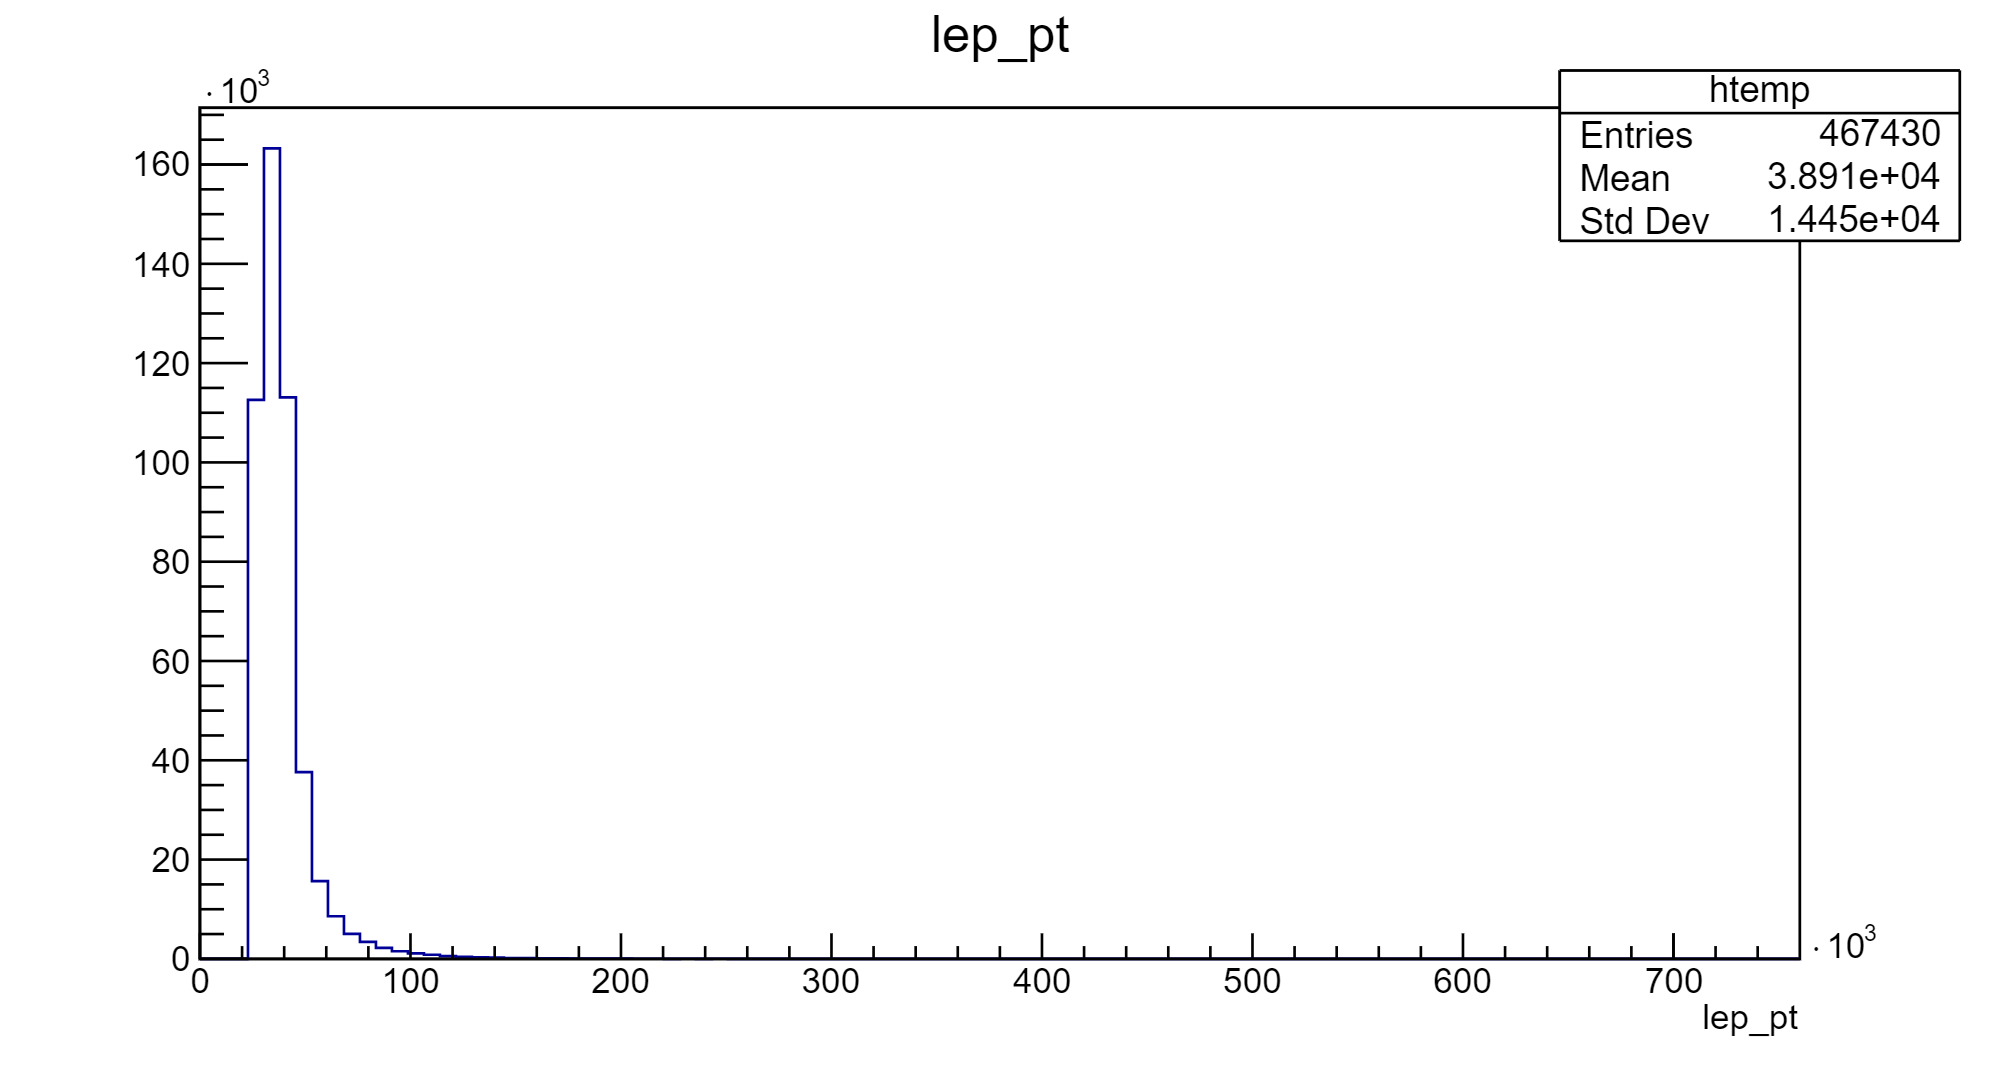
\includegraphics[width=\linewidth]{plots/TB_lep_pt.png}
    \caption{Distribution fo the transversal momentum of the lepton. This plot is a screenshot taken from the \texttt{TBrowser} in the \texttt{ROOT} enviroment. }
    \label{fig:leppt}
\end{figure}


\subsection{Event selection}
\label{sec:aufgabe3}
The chosen channel in this analysis is the \texttt{lepton+jets} channel where exactly one charged lepton is produced via $W$ boson decays.
A minimum transversal momentum of $\texttt{lep$\_$pt} \textgreater \SI{50}{\giga\electronvolt}$ is recommended for this lepton.
Events that include a lepton with a smaller transversal momentum are being removed.
This process also includes a neutrino which cannot be observed by the detector, so that a missing transversal energy of $\texttt{met$\_$et} \textgreater \SI{40}{\giga\electronvolt}$ is required as well.
Since both top quarks decay into a bottom quark and  a $W$ boson, at least a jet number of $\texttt{jet$\_$n} \textless 4$ is required in the selection because of one $W$ boson decaying into two quarks as well.
Two of these jets have to be b-tagged.
A $\texttt{jet$\_$pt} \textgreater \SI{40}{\giga\electronvolt}$ is recommended for all jets and at least one with a $\texttt{lep$\_$pt} \textgreater \SI{100}{\giga\electronvolt}$.
Because of the detector acceptance, the pseudorapidity is set to a value of $|{\eta}| \textless 2.5$. \par

The coefficient $\epsilon \cdot A$ (efficiency times detector acceptance) is calculated as the ratio of events after each of the different requirements in the event selection to the total number of events in the sample.

The efficiencies after each step as well as the corresponding sample is found in table \ref{tab:eff}.
Cuts on the pseudorapidity of the lepton and the jets are made after $\texttt{lep$\_$pt}$ and $\texttt{jet$\_$pt}$.
These do not show any significant change in the efficiency of any sample, thus they are not shown in the table.

\begin{table}
    \centering
    \caption{Calculated efficiencies after cutting on different variables.}
    \label{tab:eff}
    \resizebox{\textwidth}{!}{\begin{tabular}{c|cccccc}
    \toprule
    Sample & $\texttt{lep$\_$n}$ & $\texttt{lep$\_$pt}$  & $\texttt{jet$\_$n}$ & $\texttt{jet$\_$pt}$ & $\texttt{btagged}$ & $\texttt{met$\_$et} $   \\
    \midrule
    \texttt{ttbar.el}      & 0.9316 & 0.5070  & 0.2440 & 0.1408  & 0.0606      & 0.0430\\
    \texttt{ttbar.mu}      & 0.9200 & 0.4821  & 0.2328 & 0.1342  & 0.0580      & 0.0410\\
    \texttt{singletop.el}  & 0.9806 & 0.4323  & 0.0532 & 0.0311  & 0.0103      & 0.0071\\
    \texttt{singletop.mu}  & 0.9786 & 0.4104  & 0.0498 & 0.0288  & 0.0097      & 0.0068\\
    \texttt{diboson.el}    & 0.9044 & 0.3813  & 0.0119 & 0.0048  & 0.0001      & 7.9691e-05 \\
    \texttt{diboson.mu}    & 0.8731 & 0.3510  & 0.0091 & 0.0038  & 9.99691e-05 & 7.38902e-05 \\
    \texttt{wjets.el}      & 0.9999 & 0.1709  & 0.0029 & 0.0017  & 1.99407e-05 & 1.39121e-05\\
    \texttt{wjets.mu}      & 0.9999 & 0.1589  & 0.0027 & 0.0016  & 2.33554e-05 & 1.56505e-05\\
    \texttt{zjets.el}      & 0.7167 & 0.1814  & 0.0067 & 0.0032  & 0.000135906 & 4.8692e-05\\
    \texttt{zjets.mu}      & 0.5015 & 0.1256  & 0.0025 & 0.0014  & 7.37231e-05 & 3.18146e-05\\
    \texttt{zprime400.el}  & 0.9308 & 0.4464  & 0.1640 & 0.0470  & 0.0192      & 0.0124\\
    \texttt{zprime400.mu}  & 0.9201 & 0.4215  & 0.1597 & 0.0539  & 0.0203      & 0.0137\\
    \texttt{zprime500.el}  & 0.9324 & 0.5616  & 0.2539 & 0.1501  & 0.0626      & 0.0418\\
    \texttt{zprime500.mu}  & 0.9224 & 0.5353  & 0.2319 & 0.1358  & 0.0581      & 0.0389\\
    \texttt{zprime750.el}  & 0.9237 & 0.6705  & 0.3881 & 0.3503  & 0.1573      & 0.1216\\
    \texttt{zprime750.mu}  & 0.9133 & 0.6451  & 0.3710 & 0.3332  & 0.1526      & 0.1220\\
    \texttt{zprime1000.el} & 0.9339 & 0.7342  & 0.4599 & 0.4401  & 0.2088      & 0.1790\\
    \texttt{zprime1000.mu} & 0.9182 & 0.7055  & 0.4573 & 0.4335  & 0.2023     & 0.1682\\
    \texttt{zprime1250.el} & 0.9355 & 0.7475  & 0.4811 & 0.4667  & 0.2158      & 0.1900 \\
    \texttt{zprime1250.mu} & 0.9246 & 0.7319  & 0.4867 & 0.4704  & 0.2218      & 0.1932\\
    \texttt{zprime1500.el} & 0.9401 & 0.7711  & 0.5014 & 0.4904  & 0.2121      & 0.1904\\
    \texttt{zprime1500.mu} & 0.9287 & 0.7483  & 0.5012 & 0.4906  & 0.2126      & 0.1894\\
    \texttt{zprime1750.el} & 0.9473 & 0.7758  & 0.5140 & 0.5038  & 0.2146      & 0.1932\\
    \texttt{zprime1750.mu} & 0.9383 & 0.7571  & 0.5036 & 0.4918  & 0.2091      & 0.1898\\
    \texttt{zprime2000.el} & 0.9451 & 0.7629  & 0.4988 & 0.4876  & 0.1914     & 0.1749\\
    \texttt{zprime2000.mu} & 0.9406 & 0.7611  & 0.5171 & 0.5069  & 0.1971      & 0.1802\\
    \texttt{zprime2250.el} & 0.9450 & 0.7451  & 0.4948 & 0.4841  & 0.1846      & 0.1688\\
    \texttt{zprime2250.mu} & 0.9448 & 0.7640  & 0.5183 & 0.5086  & 0.2012      & 0.1824\\
    \texttt{zprime2500.el} & 0.9480 & 0.7509  & 0.4958 & 0.4811  & 0.1762      & 0.1600\\
    \texttt{zprime2500.mu} & 0.9433 & 0.7595  & 0.5211 & 0.5080  & 0.1933      & 0.1765\\
    \texttt{zprime3000.el} & 0.9437 & 0.7151  & 0.4510 & 0.4268  & 0.1656      & 0.1463\\
    \texttt{zprime3000.mu} & 0.9398 & 0.7314  & 0.4833 & 0.4633  & 0.1781      & 0.1607\\
    \bottomrule
    \end{tabular}}
\end{table}

After this event selection $t\bar{t}$ prodiction is the dominant background since it has a very similar final state as the signal channel.


\subsection{Fundamental distributions}
The dominant background process is the $t\bar{t}$ production.
In the following, distributions of variables of simulated $t\bar{t}$ Monte Carlo events with muons are shown and compared to the expected distribution.
Some of these distriutions are shown in figure \ref{fig:distriutions}.
These are in agreement with the expected distributions of these variables.
In figure \ref{fig:btagged}, the number of b-tagged jets in each event is shown.
Figure \ref{fig:decay} shows the production of two bottom quarks so that most likely two jets are b-tagged.
This expectation is in agreement with figure \ref{fig:btagged}.
The remaining momentum that is not in the jets is evenly split on the muon and the neutrino.
The distributions of the $\texttt{lep$\_$pt}$ and $\texttt{met$\_$et}$ is very similar.
Both have their respective peak at the same location.
The $\texttt{met$\_$et}$ is more smeared out since the indirect measured neutrinos have a worse resolution.
Besides that these variables follow their expected distributions.

\begin{figure}
  \begin{subfigure}{0.5\textwidth}
    \centering
    \includegraphics[width=\linewidth]{plots/ttbar.mu_selected_lep_pt.pdf}
    \caption{}
    \label{fig:lep_pt}
  \end{subfigure}%
  \begin{subfigure}{0.5\textwidth}
    \centering
    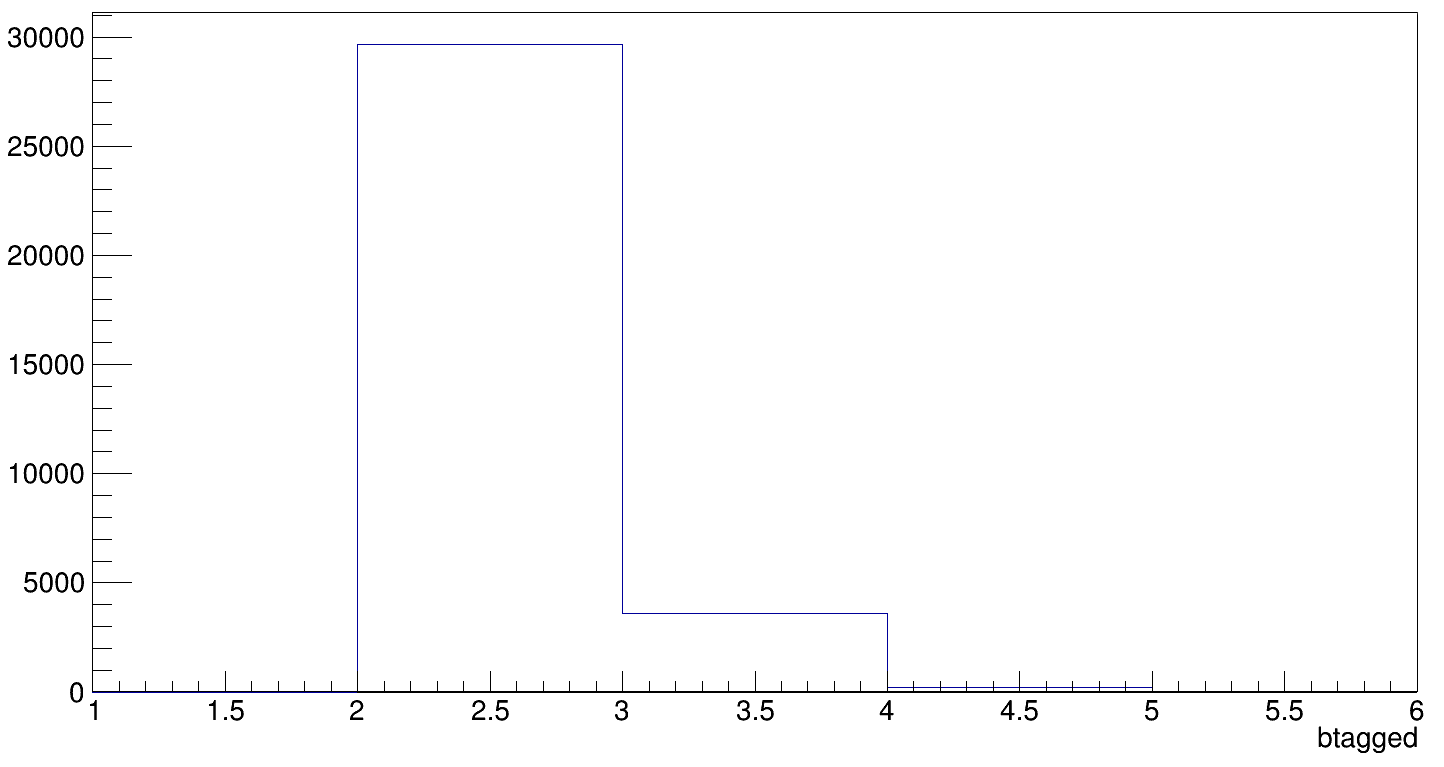
\includegraphics[width=\linewidth]{plots/btagged.png}
    \caption{}
    \label{fig:btagged}
  \end{subfigure}%
  \newline
  \begin{subfigure}{0.5\textwidth}
    \centering
    \includegraphics[width=\linewidth]{plots/ttbar.mu_selected_jet_pt.pdf}
    \caption{}
    \label{fig:jet_pt}
  \end{subfigure}%
  \begin{subfigure}{0.5\textwidth}
    \centering
    \includegraphics[width=\linewidth]{plots/ttbar.mu_selected_met_et.pdf}
    \caption{}
    \label{fig:met_et}
  \end{subfigure}%
  \caption{Plots of different variables of the $t\bar{t}$ Monte Carlo simulations.
  The following variables are shown here: The transversal momentum of the lepton (\subref{fig:lep_pt}), the amount of b-tagged jets (\subref{fig:btagged}), the transversal momentum of the jets (\subref{fig:jet_pt}) and the missing transversal energy (\subref{fig:met_et}).
  }
  \label{fig:Distributions}
\end{figure}

\subsection{Derived quantities}

After the event selection, some background processes like $t\bar{t}$ events are still not negligible.
To have a better discrimination, some quantities are being computed that might increase the seperation power between $Z^\prime$ and $t\bar{t}$ events. The following quantities were computed and compared in $Z^\prime$ and $t\bar{t}$ events:
\begin{itemize}
 \item the difference of the azimuth angle of the missing transversal energy and the lepton flight direction $\Delta\Phi$
 \item the invariant mass of the system formed by the three jets with the largest transversal momentum
 \item the invariant mass and the pseudorapidity of the system formed by the four jets with the largest momentum, the muon and the neutrino
\end{itemize}
To calculate the invariant mass of the system including neutrinos, the class \texttt{TLorentzVektor} was used to compute the four-vector information.
While calculating $\Delta\Phi$, only the smaller difference of $|\phi_1 - \phi_2|$ and $|2\pi - |\phi_1 - \phi_2|$ was used.
These quantities were calculated for all data and Monte Carlo samples.
To determine the quantity with the largest separation power, the dominant background ($t\bar{t}$) is compared with a possible signal ($Z^\prime(1000)$).
The best discriminate is the invariant mass of the full system.
This quantity is shown in figure \ref{fig:Comparison} for $t\bar{t}$ and $Z^\prime(1000)$.

\begin{figure}
  \begin{subfigure}{0.5\textwidth}
    \centering
    \includegraphics[width=\linewidth]{plots/ttbar.mu_selected_SysJetMass.pdf}
    \caption{}
    \label{fig:ttbar_sys}
  \end{subfigure}%
  \begin{subfigure}{0.5\textwidth}
    \centering
    \includegraphics[width=\linewidth]{plots/zprime1000.mu_selected_SysJetMass.pdf}
    \caption{}
    \label{fig:zprime_sys}
  \end{subfigure}%
  \caption{Distribution of the chosen discrimination quantity, the invariant mass of the system formed by the four jets with the largest transversal momentum, the muon and the neutrino.
This quantity is shown for $t\bar{t}$ simulations (\subref{fig:ttbar_sys}) and simulations of  $Z^\prime(1000)$ (\subref{fig:zprime_sys}).
  }
  \label{fig:Comparison}
\end{figure}


\section{Agreement between data and simulation}
After the selection is done, the agreement of data and simulation is investigated.
For that, the expected amount of event is being calculated using the formula
\begin{equation}
N = \mathcal{L} \sigma (A \epsilon)\,.
\label{eqn:erwartung}
\end{equation}
Here $(A \cdot \epsilon)$ is the acceptance times the efficiency of the event selection that was calulated in section \ref{sec:aufgabe3}, $\sigma$ is the cross section of the respective event and $\mathcal{L} = \SI{1}{\femto b}^{-1}$ is the integrated luminosity of the dataset.
Cross sections as well as expected amount of events in the chose data sample (\texttt{data.mu.2.root}) are shown in table \ref{tab:Erwartungen}.
A total amount of $70.42$ background events is expected in this sample. After selection, the total amount of events is $N_{tot} = 99$.
\begin{table}[H]
    \centering
    \caption{Anzahl erwarteter Ereignisse für die einzelnen Prozesse im sample \texttt{data.mu.2.root}. Angegeben
    ist der zugehörige Wirkungsquerschnitt der für die Berechnung der einzelnen Werte nach Formel
    \eqref{eqn:erwartung} benötigt wird.}
    \label{tab:Erwartungen}
    \begin{tabular}{c|cc}
    \toprule
    Prozess & $\text{N}_\text{expected}$ & $\sigma$ / $\SI{}{\pico b}$ \\
    \midrule
    \texttt{ttbar}      &  3.1893  & 252.82    \\
    \texttt{singletop}  &  3.5362   & 52.47     \\
    \texttt{diboson}    &  3.1561   & 29.41     \\
    \texttt{zjets}      &  6.6564   & 2516.20   \\
    \texttt{wjets}      &  53.8832  & 36214     \\
    \texttt{zprime400}  &  108.9000 & 1.1e2     \\
    \texttt{zprime500}  &  81.1800  & 8.2e1     \\
    \texttt{zprime750}  &  19.8000  & 2.0e1     \\
    \texttt{zprime1000} &  5.4450  & 5.5       \\
    \texttt{zprime1250} &  1.881 & 1.9       \\
    \texttt{zprime1500} &  0.8217   & 8.3e-1    \\
    \texttt{zprime1750} &  0.2970   & 3.0e-1    \\
    \texttt{zprime2000} &  0.1386   & 1.4e-1    \\
    \texttt{zprime2250} &  0.0663  & 6.7e-2    \\
    \texttt{zprime2500} &  0.0346   & 3.5e-2    \\
    \texttt{zprime3000} &  0.0119   & 1.2e-2    \\
    \bottomrule
    \end{tabular}
\end{table}

For these events, weights need to be applied since they are just refering to their respective sample.
These weights normalize the MC samples to the data sample.
The weights are calculated after
\begin{equation}
w = \frac{\mathcal{L} \sigma}{\text{N}_\text{MC}}\,.
\label{eqn:weights}
\end{equation}
$\text{N}_\text{MC}$ is the number of MC events before the preselection.
The sizes of the samples as well as the calculated weights are shown in table \ref{tab:weights}.

\begin{table}[H]
    \centering
    \caption{Calculated weights for the different processes. The cross section used to calculate the weights is shown in table  \ref{tab:Erwartungen}. The integrated luminosity is $\mathcal{L} = \SI{1}{\femto b}^{-1}$. The weights are calculated using \eqref{eqn:weights}.}
    \label{tab:weights}
    \begin{tabular}{c|cc}
    \toprule
    process & $\text{N}_\text{MC}$ & weights $w$ \\
    \midrule
    \texttt{ttbar}      & 7847944    & 0.03221     \\
    \texttt{singletop}  & 1468942    & 0.03572     \\
    \texttt{diboson}    & 922521     & 0.03188     \\
    \texttt{wjets}      & 66536222   & 0.54428     \\
    \texttt{zjets}      & 37422926   & 0.06724     \\
    \texttt{zprime400}  & 100000     & 1.10000     \\
    \texttt{zprime500}  & 100000     & 0.82000     \\
    \texttt{zprime750}  & 100000     & 0.20000     \\
    \texttt{zprime1000} & 100000     & 0.55000     \\
    \texttt{zprime1250} & 100000     & 0.19000     \\
    \texttt{zprime1500} & 100000     & 0.08300     \\
    \texttt{zprime1750} & 100000     & 0.03000     \\
    \texttt{zprime2000} & 100000     & 0.01400     \\
    \texttt{zprime2250} & 100000     & 0.00067     \\
    \texttt{zprime2500} & 100000     & 0.00035     \\
    \texttt{zprime3000} & 100000     & 0.00012     \\
    \bottomrule
    \end{tabular}
\end{table}

After applying these weights, stacked plots are being produced.
For that the different background process distributions are stacked and the data events are added to compare them to the expected background. Four of these plots are shown in figure \ref{fig:stack}.


\begin{figure}[H]
  \begin{subfigure}{0.5\textwidth}
    \centering
    \includegraphics[width=\linewidth]{plots/stacked_lep_pt.pdf}
    \caption{}
    \label{fig:stacked_lep_pt}
  \end{subfigure}%
  \begin{subfigure}{0.5\textwidth}
    \centering
    \includegraphics[width=\linewidth]{plots/stacked_jet_eta.pdf}
    \caption{}
    \label{fig:stacked_jet_eta}
  \end{subfigure}%
  \newline
  \begin{subfigure}{0.5\textwidth}
    \centering
    \includegraphics[width=\linewidth]{plots/stacked_jet_pt.pdf}
    \caption{}
    \label{fig:stacked_jet_pt}
  \end{subfigure}%
  \begin{subfigure}{0.5\textwidth}
    \centering
    \includegraphics[width=\linewidth]{plots/stacked_lep_E.pdf}
    \caption{}
    \label{fig:stacked_lep_E}
  \end{subfigure}%
  \caption{Stacked background samples in comparison to the data sample.
Shown is the transversal momentum of the muon (\subref{fig:stacked_lep_pt}), the jet pseudorapidity (\subref{fig:stacked_jet_eta}),
  the transversal momentum of the jets (\subref{fig:stacked_jet_pt}) and lepton energy (\subref{fig:stacked_lep_E}).
  }
  \label{fig:stack}
\end{figure}

All four plots show a mostly good agreement of expected background and data.
Some data points are higher than the expected background which could be a hint on a $Z^\prime$ event.
In this case there are also some data points lower than the expected background, indicating that these are just statistical fluctuations.

Figure \ref{fig:disc} shows the discriminating variable, the invariant mass of the system.
\begin{figure}[H]
    \centering
    \includegraphics[width=\linewidth]{plots/stacked_mass.pdf}
    \caption{Distrubution of expected background events and data of the invariant mass of the system.}
    \label{fig:disc}
\end{figure}

The same properties as before can be observed in this plot. There are some data points higher than the expected background and some that are significantly lower.
This again indicates that these peaks are just statistical fluctuations.


\section{Statistical analysis}
In the last chapter, the agreement between MC and data was qualitatively inspected.
To judge the agreement between data and the background-only hypothesis, a $\chi^2$ test will be performed using MC simulations as the background-only hypothesis.
The value of $\chi^2$ is a metric for the deviation of the data and MC sample.
If the background-only hypothesis  and data are in a good agreement, meaning no $Z^\prime$ exists, $\chi^2$ will have a small value.
In this case an exclusion limit will be set on the production cross section.
For that a confidence level is needed that is calculated with
\begin{equation}
  \text{CL}= 1-p
\end{equation}
with $p$ as the $p$-value for the background-only hypothesis.

The results of the $\chi^2$ test are:
\begin{align*}
  \chi^2= 25.1862 \\
  p = 0.508458
\end{align*}
Even though a high $\chi^2$ value is achieved, the $p$-value is very high as well.
This shows that the found peaks in the invariant mass is just a statistical fluctuation and that no observation of a $Z^\prime$ is found.
Therefore an exclusion limit for the different $Z^\prime$ mass hypotheses will be calculated in a $\SI{95}{\percent}$ confidence level.
To consider the weights, a scaler will be used that scales the weights until the confidence level is reached.
These results are shown in table \ref{tab:chi2}.

\begin{table}
  \centering
  \caption{Calculated parameters of the $\chi^2$ test for the different  $Z^\prime$ mass hypothises as well as the cross section exclusion limit in a  $\SI{95}{\percent}$ confidence level.}
  \label{tab:chi2}
  \begin{tabular}{c|cccc}
    \toprule
    process & degrees of freedom & $p$-value & scaler & $\sigma / \si{\pico b}$ \\
    $Z^\prime (400)$  & 26 & 0.00549806 & 0.4 & 44 \\
    $Z^\prime (500)$  & 26 & 0.00211708 & 0.2 & 16.4 \\
    $Z^\prime (750)$  & 26 & 0.0150853  & 0.2 & 4 \\
    $Z^\prime (1000)$ & 26 & 0.0472768 & 0.4 & 2.2 \\
    $Z^\prime (1250)$ & 26 & 0.0394068 & 0.9 & 1.71 \\
    $Z^\prime (1500)$ & 26 & 0.0433432 & 1.9 & 1.58 \\
    $Z^\prime (1750)$ & 26 & 0.0462103 & 4.8 & 1.44 \\
    $Z^\prime (2000)$ & 26 & 0.0499252 & 10.9 & 1.526 \\
    $Z^\prime (2250)$ & 26 & 0.0495314 & 23.5 & 1.57 \\
    $Z^\prime (2500)$ & 26 & 0.0498703 & 48.7 & 1.70 \\
    $Z^\prime (3000)$ & 26 & 0.0499869  & 194.7 & 2.33 \\
    \midrule
    \bottomrule
  \end{tabular}
\end{table}

The resulting cross section at the $\SI{95}{\percent}$ confidence level are being compared against the expected cross sections in figure \ref{fig:limit}.
Since the observed cross section is smaller than theoretically predicted, masses of $m_{Z^\prime} \textless \SI{1300}{\giga\electronvolt}$ can be excluded.
A particle with a lower mass would have been observed in this analysis.
Masses of $m_{Z^\prime} \textgreater \SI{1300}{\giga\electronvolt}$ could not be discriminated from the background so that these masses are not excluded in this analysis.

\begin{figure}
    \centering
    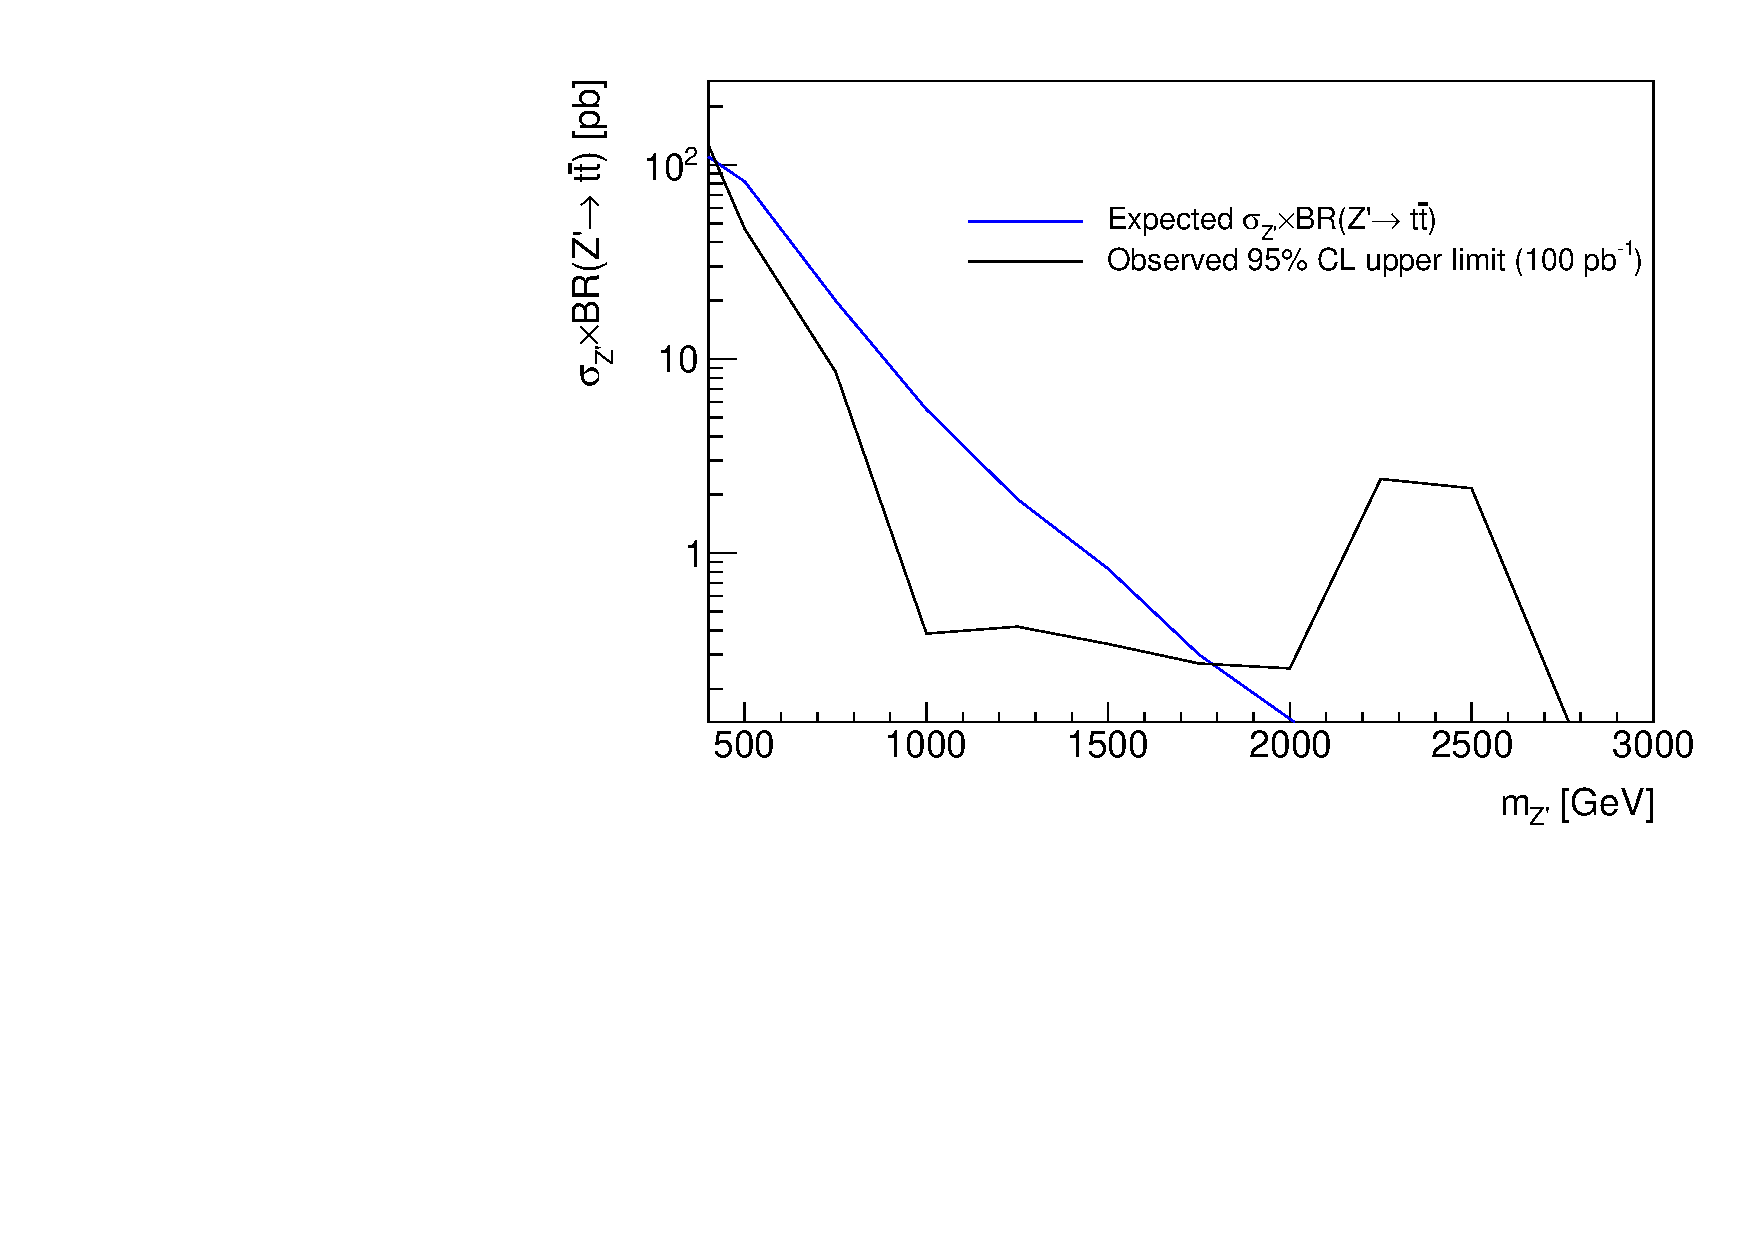
\includegraphics[width=\linewidth]{plots/limits.pdf}
    \caption{Calculated upper limits of the cross section in a $\SI{95}{\percent}$ confidence level for the different $Z^\prime$ mass hypothises. For comparison, the expected cross section is plotted as well.}
    \label{fig:limit}
\end{figure}

